\chapter{若当标准形}

本讲我们将在前面讨论的基础上实现复数域上相似标准形理论的终极目标,即得到复数域上全体线性变换都可以得到的一种比较简单的矩阵表示——若当标准形. 我们将讨论其存在与唯一性,并在证明唯一性的过程中给出一种求解若当标准形的方法. 最后,我们将讨论若当标准形的应用.

\section{若当标准形的存在性}
回顾\autoref{thm:15:不变子空间与分块对角矩阵},我们知道寻找线性变换$T\in\mathcal{L}(V)$在基下简单的表示矩阵的一般思路是将$V$分解为一系列不变子空间的直和. 在对角化一节中我们尝试分解为一维不变子空间的直和,但这并不能对所有的线性变换都成立,于是我们进一步在\autoref{thm:16:广义特征性质}中对于任意的线性变换都利用广义特征子空间实现了这一分解,这也直接导出了\autoref{thm:16:分块对角矩阵}中的分块对角形矩阵表示. 然而我们仍无法满足于将这一矩阵表示作为标准形,因为我们还希望分块对角矩阵中每个分块都要足够简单,即有一定的规律且有较多的零元素,所以我们需要对广义特征子空间做进一步的分解,并且取特定形式的基来实现这一目标. 我们首先看如下例子:

\begin{example}
    设$\sigma\in\mathcal{L}(\mathbf{C})^6$满足
    \[\sigma(x_1,x_2,x_3,x_4,x_5,x_6)=(2x_1+x_2,2x_2+x_3,2x_3,2x_4,3x_5+x_6,3x_6),\]
    则我们很容易写出其在$(\mathbf{C})^6$自然基下的矩阵表示为
    \[\left(\begin{array}{ccc:c:cc}
        2 & 1 & 0 & 0 & 0 & 0\\
        0 & 2 & 1 & 0 & 0 & 0\\
        0 & 0 & 2 & 0 & 0 & 0\\
        \hdashline
        0 & 0 & 0 & 2 & 0 & 0\\
        \hdashline
        0 & 0 & 0 & 0 & 3 & 1\\
        0 & 0 & 0 & 0 & 0 & 3\\
        \end{array}\right)\]
\end{example}

通过这一例子我们观察到线性变换的一种分块对角矩阵表示,其中每个分块都十分简单,很适合作为我们实现为复数域上任意线性变换寻找的标准形. 我们称如上例矩阵表示的每个分块的形式的矩阵为\term{若当块}\index{ruodangkuai@若当块 (Jordan block)},更严谨地,域$\mathbf{F}$上的一个$r$级矩阵形如\[\begin{pmatrix}
    \lambda & 1 &        &   \\
      & \lambda & \ddots &   \\
      &   & \ddots & 1 \\
      &   &        & \lambda
\end{pmatrix}\]
则称其为一个$r$级若当块(1级显然就是1阶矩阵),记作$J_r(\lambda)$,其中$\lambda$是对角线上元素. 若一个线性变换$\sigma$在基$B$下的矩阵表示是对角块均为若当块的分块对角矩阵,则称这个分块对角矩阵是线性变换$\sigma$的\term{若当标准形}\index{ruodangxing@若当标准形 (Jordan canonical form)},而这组基$B$称为$T$的\term{若当基}\index{ruodangji@若当基 (Jordan basis)}. 我们希望复数域上任意线性变换都能找到一组若当基使其矩阵表示为若当标准形,而这正是本节需要证明的目标.

为了证明这一结果,我们需要首先观察若当块能在怎样的基下表示出. 为了发现这一规律,我们考虑一种最简单的情况,即一个线性变换$T$在某组基$B=\{v_1,v_2,v_3,\cdots,v_n\}$下的矩阵表示就是一个若当块,即
\[\sigma(v_1,v_2,v_3,\cdots,v_n)=(v_1,v_2,v_3,\cdots,v_n)\begin{pmatrix}
    \lambda & 1 &        &   \\
      & \lambda & \ddots &   \\
      &   & \ddots & 1 \\
      &   &        & \lambda
\end{pmatrix},\]
所以我们根据线性映射矩阵表示的定义可以得到
\begin{align*}
    \sigma(v_1)&=\lambda v_1,\\
    \sigma(v_2)&=\lambda v_2+v_1,\\
    \sigma(v_3)&=\lambda v_3+v_2,\\
    &\cdots\\
    \sigma(v_n)&=\lambda v_n+v_{n-1}.
\end{align*}

我们稍作变换,可以得到
\begin{equation} \label{eq:17:若当基的推导}
    \begin{aligned}
        (\sigma-\lambda I)v_1&=0,\\
        (\sigma-\lambda I)v_2&=v_1,\\
        (\sigma-\lambda I)v_3&=v_2,\\
        &\cdots\\
        (\sigma-\lambda I)v_n&=v_{n-1}.
    \end{aligned}
\end{equation}

即我们需要的这组基实际上具有如下形式:
\[B=\{(\sigma-\lambda I)^{n-1}(v_n),(\sigma-\lambda I)^{n-2}(v_n),\cdots,(\sigma-\lambda I)(v_n),v_n\},\]
并且有$(\sigma-\lambda I)^n=0$. 事实上观察上面这组等式,从第一个式子我们知道$v_1$实际上是$\sigma$关于特征值$\lambda$的特征向量,$v_2,\cdots,v_n$则是关于特征值$\lambda$的广义特征向量.

再进一步观察这样的一组向量,我们发现这组向量似乎与\autoref{thm:15:循环子空间}中提到的循环基有些类似:它们都是从一个向量开始,不断作用一个线性变换等到的一组向量. 这里我们给出一个定义来详细地说明一些术语:
\begin{definition} \label{def:17:若当循环基}
    设$\sigma\in\mathcal{L}(V)$,$v\in V$是关于特征值$\lambda\in\mathbf{C}$的一个广义特征向量. 设$n$是使得$(\sigma-\lambda I)^n v=0$成立的最小正整数,则称$\{(\sigma-\lambda I)^{n-1}(v),(\sigma-\lambda I)^{n-2}(v),\cdots,(\sigma-\lambda I)(v),v\}$是\term{$\sigma$关于特征值$\lambda$的循环广义特征向量组}(不引起歧义的情况下也可称循环向量),其中$(\sigma-\lambda I)^{n-1}(v)$称为其起始向量,$v$称为其终止向量.
\end{definition}

给出这一定义后,便可以开始研究这一组向量与我们目标中的若当基之间的关联. 我们需要暂时停下前进的脚步,仔细思考我们需要什么. 我们的最终目标是证明,对于任意复向量空间上的线性变换,都能找到一组基,其矩阵表示为分块对角矩阵,且每一对角块为若当块. 根据\autoref{thm:15:不变子空间与分块对角矩阵},我们要求每个若当块对应的基向量张成的子空间是不变子空间,因为这样才能保证生成一个对角块. 而根据之前的推导,我们知道生成若当块必须要这样的一组循环向量,那么自然地我们会有两个问题:
\begin{enumerate}
    \item 循环向量生成的子空间一定是不变子空间吗?因为这样才能保证生成一个对角块;
    \item 我们是从一组基$v_1,\cdots,v_n$可以得到若当块出发定义出这样的循环向量的,那么是不是一组向量满足这样的定义也一定线性无关的呢?因为这样只需要找到这样一组循环向量就一定可以构成若当基的一部分.
\end{enumerate}
事实上如果读者熟悉之前讨论的一些例子和性质,这两个问题可以轻松解决:
\begin{theorem} \label{thm:17:若当循环基的性质}
    设$\sigma\in\mathcal{L}(V)$,$B$是$\sigma$关于特征值$\lambda$的循环广义特征向量组,则
    \begin{enumerate}
        \item $B$是线性无关的,因此可以构成$\spa(B)$的一组基,称其为一组\term{若当循环基};
        \item $B$生成的子空间$W$是$\sigma$的不变子空间(就是\autoref{def:15:循环子空间}定义的循环子空间).
    \end{enumerate}
\end{theorem}
\begin{proof}
    \begin{enumerate}
        \item 由$B$的生成过程\autoref{eq:17:若当基的推导}和\autoref{ex:15:特征向量生成线性无关组},线性无关性是显然的推论.
        \item 由$B$的定义(注意$(\sigma-\lambda I)^n v=0$)以及\autoref{thm:15:循环子空间},$W$是$\sigma$的不变子空间.
    \end{enumerate}
\end{proof}

在以上问题被解决后,我们的目标将非常清晰,即对任意的复数域上的线性变换是否一定能找到一组基是由不同的若当循环基合并而成的,从而在在这组基下的矩阵表示是若当标准形?似乎有些困难,我们需要一些观察:事实上,若当循环基中的每个向量都是关于某个特征值$\lambda$的广义特征向量,因此它们张成的子空间应当是广义特征子空间$G_\lambda$的一部分(当然也可能张成整个广义特征子空间). 于是站在\autoref{thm:16:广义特征性质}中广义特征子空间分解的基础上,我们的目标可以转化为对其中的每一个广义特征子空间,找到一组由一个或多个若当循环基合并而成的基?这样首先利用\autoref{thm:16:广义特征性质}中广义特征子空间分解,再利用广义特征子空间的若当循环基分解,我们就可以得到一组由不同的若当循环基合并而成的基,从而得到若当标准形.

为了更清晰地展示,我们将上述过程形式化. 设$\sigma\in\mathcal{L}(V)$,$\lambda_1,\cdots,\lambda_m$是$\sigma$的互异特征值,$G_{\lambda_i}$是关于特征值$\lambda_i$的广义特征子空间. 根据\autoref{thm:16:广义特征性质},我们知道
\[V=G_{\lambda_1}\oplus\cdots\oplus G_{\lambda_m}=\mathop{\oplus}\limits_{i=1}^m G_{\lambda_i},\]
然后我们希望为每个广义特征子空间选取一组由一个或多个若当循环基合并而成的基,也就是说我们希望将每个广义特征子空间分解为一个或多个循环子空间的直和. 形式化而言,我们希望每个广义特征子空间$G_{\lambda_i}$可以由$s_i$组若当循环基$B_{i1},B_{i2},\cdots,B_{is_i}$张成,其中每一组基都可以表达为:
\[B_{ij}=\{(\sigma-\lambda_iI)^{r_{ij}-1}(v_{ij}),(\sigma-\lambda_iI)^{r_{ij}-2}(v_{ij}),\cdots,v_{ij}\},\]
事实上$r_{ij}$就是这组若当循环基的长度. 我们设由$B_{ij}$张成的循环子空间为$C_{ij}$,则有
\[G_{\lambda_i}=C_{i1}\oplus C_{i2}\oplus\cdots\oplus C_{is_i}=\mathop{\oplus}\limits_{j=1}^{s_i} C_{ij},\]
再结合\autoref{thm:16:广义特征性质}的分解,我们有
\begin{equation} \label{eq:17:循环子空间分解}
    V=\mathop{\oplus}\limits_{i=1}^m G_{\lambda_i}=\mathop{\oplus}\limits_{i=1}^n\mathop{\oplus}\limits_{j=1}^{s_i} C_{ij}.
\end{equation}

根据\autoref{thm:17:若当循环基的性质},每个循环子空间都是不变子空间,并且每个若当循环基都对应于一个若当块. 回忆我们上面的推导过程,我们现在剩下的任务就是为复数域上的任意广义特征子空间$G_{\lambda_i}$找到一组由一个或多个若当循环基合并而成的基,这样就能得到\autoref{eq:17:循环子空间分解}所示的分解,从而得到任意复数域上的线性变换都存在若当标准形. 为了实现这一目标,我们需要先证明一个关于若当循环基的性质.

\begin{lemma} \label{lem:17:若当循环基合并性质}
    设$\sigma\in\mathcal{L}(V)$,$\lambda\in\mathbf{C}$是$\sigma$的一个特征值. 设$B_1,\cdots,B_q$都是$\sigma$关于特征值$\lambda$的一组若当循环基,且它们的起始向量各不相同且构成了一组线性无关向量组,则
    \begin{enumerate}
        \item $B_i(i=1,\cdots,q)$是互不相交的;
        \item $B=B_1\cup\cdots\cup B_q$是线性无关向量组.
    \end{enumerate}
\end{lemma}
\begin{proof}
    \begin{enumerate}
        \item 反证法. 假设$B_i$和$B_j$有交集,即存在$v\in B_i\cap B_j$. 设$B_i$和$B_j$的终止向量分别为$v_i$和$v_j$,则存在非负整数$m_i,m_j$使得
        \[(\sigma-\lambda I)^{m_i}(v_i)=(\sigma-\lambda I)^{m_j}(v_j)=v.\]
        故$(\sigma-\lambda I)^{m_i+m}(v_i)=(\sigma-\lambda I)^{m_j+m}(v_j)$,其中$m$是任意非负整数,因此$B_i$和$B_j$从向量$v$开始一直到起始向量必定都是相等的,而这与定理的前提起始向量各不相同矛盾,故$B_i(i=1,\cdots,q)$是互不相交的.

        \item 同样反证法,假设$B$是线性相关向量组,则一定存在一个子向量组$u_1,\cdots,u_s$,使得有全部非零的$k_1,\cdots,k_s$使得
        \begin{equation} \label{eq:17:若当循环基合并性质证明}
            k_1u_1+\cdots+k_su_s=0.
        \end{equation}
        这是一定能做到的,因为$B$线性相关表明存在一个向量$u_1$能被其它向量线性表示,我们写出这一线性表示,去除表示中系数为0的向量,又$u_1\neq 0$,故一定剩余一组向量满足
        \[u_1=c_2u_2+\cdots+c_su_s,\]
        其中$c_i\neq 0$,则$-u_1+c_2u_2+\cdots+c_su_s=0$,这就满足\autoref{eq:17:若当循环基合并性质证明}中$k_1,\cdots,k_s$全部非零.

        接下来我们可以对每个$u_i$作用$(\sigma-\lambda I)$的幂次,在经过某个幂次后,所有的$u_i$都会变成它所在的$B_j$的起始向量. 假设每个$u_i$在作用$(\sigma-\lambda I)^{r_i}$次后变成所在$B_j$的起始向量,我们取$r=\max\{r_1,\cdots,r_s\}$,然后在\autoref{eq:17:若当循环基合并性质证明}两边作用$(\sigma-\lambda I)^r$,则可以得到
        \begin{equation}
            k_{i_1}(\sigma-\lambda I)^r(u_{i_1})+\cdots+k_{i_t}(\sigma-\lambda I)^r(u_{i_t})=0,
        \end{equation}
        其中$u_{i_1},\cdots,u_{i_t}$是$u_1,\cdots,u_s$中在作用$(\sigma-\lambda I)^r$后变成对应起始向量的向量,即$(\sigma-\lambda I)^r(u_{i_j})$都是起始向量,而其它向量已经到达超出起始向量所需次数,因此被化零. 又$k_{ij}$全都不为0,因此这些起始向量$(\sigma-\lambda I)^r(u_{i_j})$线性相关,这与定理的前提起始向量线性无关矛盾,故$B$是线性无关向量组.
    \end{enumerate}
\end{proof}

接下来我们便可以证明本节最核心的一个结果,即复数域上任意一个广义特征子空间都有一组由互不相交的循环基并起来构成的基,从而我们可以进一步利用广义特征子空间分解得到每个线性变换都有一组基使得其矩阵表示为若当标准形:
\begin{theorem} \label{thm:17:广义特征子空间分解若当基}
    设$V$是$\mathbf{C}$上的有限维线性空间,$\sigma\in\mathcal{L}(V)$,$G_\lambda$是关于特征值$\lambda$的广义特征子空间,则$G_\lambda$有一组由不相交的若当循环基取并集构成的基.
\end{theorem}
\begin{proof}
    我们对$G_\lambda$的维数进行归纳. 维数等于1时结论显然成立. 我们假设对于维数小于$n$的情况结论成立,现在考虑$G_\lambda$维数为$n$的情况,由于使用归纳法,我们需要构造出一个维数更低的广义特征子空间. 我们考虑限制线性变换$(\sigma-\lambda I)\vert_{G_\lambda}$,我们知道这一定不是单射,因为$\lambda$是$\sigma$的特征值,因此$(\sigma-\lambda I)v=0$在$G_\lambda$内一定有非零向量解(实际上就是特征向量),因此由\autoref{thm:6:双射等价条件},这也不是满射,因此$\dim\im(\sigma-\lambda I)\vert_{G_\lambda}<\dim G_\lambda$.

    我们记$U=\im(\sigma-\lambda I)\vert_{G_\lambda}$,这是一个维数更低的子空间,现在我们需要说明它是某个线性变换的广义特征子空间. 事实上我们可以直接考虑$\sigma\vert_U$,因为$\sigma$在全空间$V$上关于特征值$\lambda$的广义特征子空间是$G_\lambda$,因此限制在$G_\lambda$的子集上的映射$\sigma\vert_U$关于特征值$\lambda$的广义特征子空间必然就是$U$,因为对于任意的$u\in U\subset G_\lambda$,必然存在正整数$j$使得$(\sigma-\lambda I)^ju=0$. 于是根据归纳假设,$U$有一组由不相交的若当循环基取并集构成的基,记作$B=B_1\cup B_2\cup\cdots\cup B_q$(因为是基所以起始向量也必定线性无关).

    于是接下来我们要将这组基扩充成$G_\lambda$的一组基,并保持若当循环基的特点. 观察$U=\im(\sigma-\lambda I)\vert_{G_\lambda}$和$G_\lambda$的区别,其一在于$\sigma-\lambda I$将$G_\lambda$的一些向量映射进了$U$,但这些向量本身没能被其它向量映射到$U$中,其二在于$\sigma-\lambda I$将$G_\lambda$中的一些向量(实际上就是特征向量)化零,因此我们就从这两个角度扩充.
    \begin{enumerate}
        \item 我们考虑任一若当循环基$B_i$的终止向量,它应当是某个$v_i\in G_\lambda$在$\sigma-\lambda I$下的像,我们直接将$v_i$加入到$B_i$中,这样我们就得到了$\tilde{B_i}=B_i\cup\{v_i\},\enspace i=1,\cdots,q$,它们仍然是满足循环向量组定义的.
        \item $B$中的特征向量实际上就是每个$B_i$的起始向量,我们记为$w_1,\cdots,w_q$,它们是特征子空间$V_\lambda$的一组线性无关向量,因此可以将其扩充为$V_\lambda$的一组基
        \[w_1,\cdots,w_q,u_1,\cdots,u_s.\]
    \end{enumerate}

    从而扩张后我们得到新的一组不相交且起始向量线性无关的若当循环基的并:
    \[\tilde{B}=\tilde{B_1}\cup\tilde{B_2}\cup\cdots\cup\tilde{B_q}\cup\{u_1\}\cup\cdots\cup\{u_s\},\]

    由\autoref{lem:17:若当循环基合并性质},$\tilde{B}$必然线性无关. 最后我们证明$\tilde{B}$是$G_\lambda$的一组基. 假设$B$包含$r=\dim U$个向量,于是$\tilde{B}$包含$r+q+s$个向量. 又因为$w_1,\cdots,w_q,u_1,\cdots,u_s$是$V_\lambda$的一组基,而$V_\lambda=\ker(\sigma-\lambda I)\vert_{G_\lambda}$,由线性映射基本定理,
    \[\dim G_\lambda=\dim\ker(\sigma-\lambda I)\vert_{G_\lambda}+\dim\im(\sigma-\lambda I)\vert_{G_\lambda}=q+s+r,\]

    因此$\tilde{B}$线性无关且长度等于$G_\lambda$的维数,故是$G_\lambda$的一组若当循环基.
\end{proof}

由此,我们证明了复数域上线性变换的广义特征子空间一定有一组由若干个若当循环基合并而成的基,根据\autoref{eq:17:循环子空间分解}的推导过程,下面这一定理也就自然成立:
\begin{corollary} \label{cor:17:若当基存在}
    设$V$是$\mathbf{C}$上的有限维线性空间,$\sigma\in\mathcal{L}(V)$,则存在一组基$B$使得$\sigma$在$B$下的矩阵表示为若当标准形.
\end{corollary}

接下来我们需要描述矩阵的若当标准形. 实际上,线性变换在某组基下有若当标准形与矩阵有相似标准形为若当标准形是等价的,这一点与之前对角化、分块对角化等是一致的,因此我们很容易得到如下推论:
\begin{corollary}
    对复数域上的任意$n$阶矩阵$A$,都存在一个$n$阶矩阵$P$,使得$P^{-1}AP$是若当标准形.
\end{corollary}

至此我们已经证明对于复数域上的任意线性变换和矩阵,若当标准形的存在性,接下来我们将讨论若当标准形的唯一性,并在这一过程中讨论如何求解若当标准形和对应的基或者过渡矩阵.

\section{若当标准形的唯一性}

在上一节内容中,我们已经证明对于复数域上的任意线性变换和矩阵,都能有一组基或者过渡矩阵得到若当标准形. 本节我们将回答一个重要的问题,即一个线性变换或矩阵是否可能有两种若当基或过渡矩阵的取法,得到不同的若当标准形?我们的答案是否定的,并且在回答问题的过程中我们将给出获得这一唯一若当标准形的方法.

回忆\autoref{eq:17:循环子空间分解},我们的目标应当是为每一个广义特征子空间找到一组由若当循环基合并而成的基,然后将这些基合并成一组基,从而得到若当标准形. 因此我们只需要讨论如何对某一个特征值$\lambda$对应的广义特征子空间$G_\lambda$找到一组由一个或多个若当循环基合并而成的基即可,当一个线性变换或矩阵有多个特征值时,只需要对每一个特征值对应的广义特征子空间做同样的操作即可.

因此我们现在只考虑将映射限制于一个广义特征子空间$G_\lambda$上的情形,将该特征值对应的若当块和若当基求解出来即可. 考虑到若当基是由一系列若当循环基合并而成,而若当循环基中会出现大量的$\sigma-\lambda I$的幂次. 回忆\autoref{thm:16:广义特征性质},我们知道$(\sigma-\lambda I)\vert_{G_\lambda}$是幂零线性变换,因此我们可以自然地简记$N=\sigma-\lambda I$. 假设最终我们求得限制在$G_\lambda$下的若当基中有$n$组若当循环基,每组若当循环基的长度分别为$m_1,\cdots,m_n$(不妨设$m_1\geqslant\cdots\geqslant m_n$),则我们可以将这些若当基记为:
\[N^{m_1}v_1,\ldots,Nv_1,v_1,\ldots,N^{m_n}v_n,\ldots,Nv_n,v_n.\]

事实上这里有两组未知量,其一是每组若当循环基的长度$m_i$,这对应每个若当块的大小,因为每组若当循环基就对应于一个若当块;其二是每组若当循环基的终止向量$v_i$,这就可以决定出整个若当基. 我们接下来将分成两步来求解这两组未知量,我们将用到一个重要的工具,我们称其为\term{Young图},如\autoref{fig:17:若当基Young图形式}. 这是一种倒三角形的方格图,每一列都是一组若当循环基,按照长度从长到短依次从左到右排列,这是从列的角度看Young图.

在利用Young图求解的过程中,我们也需要从行的角度来看Young图,这时需要引入一个新的记号方便我们的求解:我们记$G_j(\lambda,\sigma)=\ker N^j$(其中$N=\sigma-\lambda I$). 根据\autoref{thm:16:核空间性质}中的核空间增长性质,我们知道当$i<j$时有$G_i(\lambda,\sigma)\subseteq G_j(\lambda,\sigma)$. 最后,在求解之前,我们需要一个引理表明下述方法的合理性:
\begin{lemma} \label{lem:17:Young图行性质}
    设$\sigma\in \mathcal{L}(V)$,若$V$中向量$v\in G_j(\lambda,\sigma)\backslash G_{j-1}(\lambda,\sigma)$,记$N=\sigma-\lambda I$,则对任意的$i<j$,有$N^iv\in G_{j-i}(\lambda,\sigma)\backslash G_{j-i-1}(\lambda,\sigma)$.
\end{lemma}

\begin{proof}
    \begin{enumerate}
        \item 直接利用定义,$v\in G_j(\lambda,\sigma)\backslash G_{j-1}(\lambda,\sigma)$表明$N^jv=0$且$N^{j-1}v\neq 0$,因此有$N^{j-i}(N^iv)=0$且$N^{j-i-1}(N^iv)\neq 0$,即$N^iv\in G_{j-i}(\lambda,\sigma)\backslash G_{j-i-1}(\lambda,\sigma)$.

        \item 与\autoref{thm:17:若当循环基的性质}理由一致,不再赘述.
    \end{enumerate}
\end{proof}

这一定理对于Young图从行来看的性质提供了一个合理性的保证. 如\autoref{fig:17:若当基Young图形式}所示,首先我们知道最上方一行是起始向量,因此都是特征向量,故这一行的向量都属于$G_1(\lambda,\sigma)$(或者$G_1(\lambda,\sigma)\backslash G_0(\lambda,\sigma)$). 然后根据\autoref{lem:17:Young图行性质},$N$的次数增加1,对应的$G_i(\lambda,\sigma)$的下标$i$就会减小1,这也就得到了\autoref{fig:17:若当基Young图形式}中每行右侧的标注的含义. 由此我们得到了Young图的行性质,接下来我们就基于Young图的行列性质求解若当基.

\begin{center}
    \textbf{\heiti 第一步\quad 求解 $\boldsymbol{m_1,\ldots,m_n}$}
\end{center}

我们首先确定每组若当循环基的长度,这一参数确定后若当形矩阵就确定了,因为每个若当循环基就对应一个若当块,因此若当循环基的长度就等于若当块的阶数,故若当形矩阵中每个若当块的大小是$(m_i+1)\times(m_i+1),\enspace i=1,\ldots,n$.
\begin{enumerate}
    \item 我们假设$m_1\geqslant\cdots\geqslant m_n$,根据前面对Young图按列和行的解读,我们将$G_\lambda$对应的若当基排列如下Young图形式(实际上图中情况对应$m_n=0$,因为$v_n$所在的若当循环基长度只有1):

    \begin{figure}[H]
        \centering
        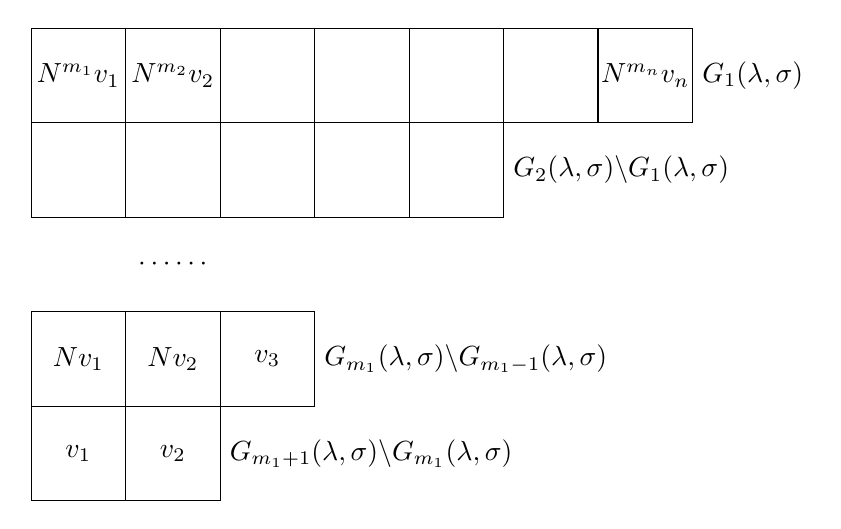
\begin{tikzpicture}
            \def\F{1.2} % scaling factor

            \foreach[count=\i] \len in {7, 7, 5, 3, 3, 2}
                \draw (0, -\F*\i+\F) -- (\F*\len, -\F*\i+\F);

            \foreach \i in {0,...,2}
                \draw (\F*\i, -3*\F) -- (\F*\i, -5*\F);
            \draw (3*\F, -3*\F) -- (3*\F, -4*\F);

            \foreach \i in {0,...,5}
                \draw (\F*\i, 0) -- (\F*\i, -2*\F);
            \foreach \i in {6,...,7}
                \draw (\F*\i, 0) -- (\F*\i, -1*\F);

            \foreach \i in {1,...,2} {
                \node at (\F*\i-.5*\F, -4.5*\F) {$v_{\i}$};
                \node at (\F*\i-.5*\F, -.5*\F) {$N^{m_{\i}}v_{\i}$};
            }
            \foreach \i in {1,...,2}
                \node at (\F*\i-.5*\F, -3.5*\F) {$Nv_{\i}$};
            \node at (3*\F-.5*\F, -3.5*\F) {$v_{3}$};
            \node at (6.5*\F, -.5*\F) {$N^{m_n}v_n$};
            \node at (1.5*\F, -2.5*\F) {$\cdots\cdots$};

            \node[anchor=west] at (7*\F, -.5*\F) {$G_1(\lambda,\sigma)$};
            \node[anchor=west] at (5*\F, -1.5*\F) {$G_2(\lambda,\sigma) \backslash G_1(\lambda,\sigma)$};
            \node[anchor=west] at (3*\F, -3.5*\F) {$G_{m_1}(\lambda,\sigma) \backslash G_{m_1-1}(\lambda,\sigma)$};
            \node[anchor=west] at (2*\F, -4.5*\F) {$G_{m_1+1}(\lambda,\sigma) \backslash G_{m_1}(\lambda,\sigma)$};
        \end{tikzpicture}
        \caption{将若当基排列成Young图形式}
        \label{fig:17:若当基Young图形式}
    \end{figure}

    \item 接下来要确定每个若当循环基的长度,也就是Young图每一列的长度,我们应当从行的性质入手,因为这是我们目前仅有的可以计算的信息. 我们需要求解每个$G_j(\lambda,\sigma)$及其维数(目前只有维数有用,但后续求解具体若当基时其中的向量也是有用的),直到某个$G_j(\lambda,\sigma)$的维数等于$G_\lambda$的维数,因为Young图中所有方格与$G_\lambda$的一组基一一对应,因此方格总数就等于$G_\lambda$的维数. 另一方面由\autoref{thm:16:广义特征性质},$N$是$G_\lambda$上的幂零线性变换,且在其它广义特征子空间上是双射,因此在核空间最高次数也只能是$G_\lambda$的维数.

    在求出各个$G_j(\lambda,\sigma)$的维数后阶梯形状也即确定,因为各层向量个数确定了. 举个简单的例子,假设$G_\lambda$是11维空间,满足$G_1(\lambda,\sigma)$,$G_2(\lambda,\sigma)$,$G_3(\lambda,\sigma)$的维数分别为5,9,11. 对照Young图每行右侧的标注,这说明从最上方一行往下的向量个数依次为5,4($=9-5$),2($=11-9$),具体Young图为
    \begin{figure}[H]
        \centering
        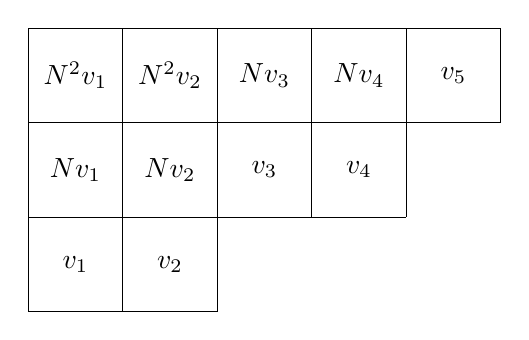
\begin{tikzpicture}
            \def\F{1.2} % scaling factor

            \foreach[count=\i] \len in {5, 5, 4, 2}
                \draw (0, -\F*\i+\F) -- (\F*\len, -\F*\i+\F);

            \foreach \i in {0,...,5}
                \draw (\F*\i, 0) -- (\F*\i, -\F);
            \foreach \i in {0,...,4}
                \draw (\F*\i, -\F) -- (\F*\i, -2*\F);
            \foreach \i in {0,...,2}
                \draw (\F*\i, -2*\F) -- (\F*\i, -3*\F);

            \node at (.5*\F, -.5*\F) {$N^2v_1$};
            \node at (1.5*\F, -.5*\F) {$N^2v_2$};
            \node at (2.5*\F, -.5*\F) {$Nv_3$};
            \node at (3.5*\F, -.5*\F) {$Nv_4$};
            \node at (4.5*\F, -.5*\F) {$v_5$};
            \node at (.5*\F, -1.5*\F) {$Nv_1$};
            \node at (1.5*\F, -1.5*\F) {$Nv_2$};
            \node at (2.5*\F, -1.5*\F) {$v_3$};
            \node at (3.5*\F, -1.5*\F) {$v_4$};
            \node at (.5*\F, -2.5*\F) {$v_1$};
            \node at (1.5*\F, -2.5*\F) {$v_2$};
        \end{tikzpicture}
    \end{figure}
    然后我们就能得到每组若当循环基的长度,即每个若当块的阶数,分别为$3,3,2,2,1$.
\end{enumerate}

基于上面的求解过程,我们就可以得到一般性的Young图大小的决定公式如下:
\begin{theorem} \label{thm:17:Young图行长度}
    令$r_j$表示Young图从上至下第$j$行的格数,则有(其中$N=\sigma-\lambda I$):
    \begin{enumerate}
    \item $r_1=\dim V-r(N)$;
    \item $r_j=r(N)^{j-1}-r(N)^j(j>1)$.
    \end{enumerate}
\end{theorem}
\begin{proof}
    根据\autoref{fig:17:若当基Young图形式}中每行右侧的标注的含义,第一行的格数就是$G_1(\lambda,\sigma)$的维数,即特征子空间的维数,即$\dim V-r(N)$;第$j(j>1)$行的格数就是$G_j(\lambda,\sigma)$的维数减去$G_{j-1}(\lambda,\sigma)$的维数,由线性映射基本定理,$\dim G_j(\lambda,\sigma)=\dim G_\lambda-r(N)^j$,$\dim G_{j-1}(\lambda,\sigma)=\dim G_\lambda-r(N)^{j-1}$,因此第$j$行的格数就是$r(N)^{j-1}-r(N)^j$.
\end{proof}

基于上述定理,我们可以进一步得到每个特征值对应的若当块个数和每个若当块大小的公式. 进一步地,这些公式实际上就表明了若当标准形的唯一性,因为每个特征值对应的若当块的个数和大小都可以被如下公式唯一确定. 我们将这一定理总结如下:
\begin{theorem} \label{thm:17:若当标准形唯一}
    设$V$是$n$维复向量空间,$\sigma\in \mathcal{L}(V)$,$\lambda_1,\ldots,\lambda_m$为其互异的特征值,记$N_j=\sigma-\lambda_j I$,则主对角元为$\lambda_j$的若当块的个数$n_j$为
    \begin{equation} \label{eq:17:若当块个数}
        n_j=n-r(N_j),
    \end{equation}
    其中$t$级若当块$J_t(\lambda_j)$的个数$n_j(t)$为
    \begin{equation} \label{eq:17:若当块大小}
        n_j(t)=r(N_j^{t+1})+r(N_j^{t-1})-2r(N_j^t),
    \end{equation}
    以上公式表明,除若当块的排列次序外,一个线性变换对应的若当标准形唯一.
\end{theorem}
\begin{proof}
    实际上,证明这一定理就是要从\autoref{thm:17:Young图行长度}中得到的Young图每行的长度推出Young图有多少列,以及每列的长度. 很显然,Young图的列数就是第一行的长度,即$\dim V-r(N_j)$. 进一步观察,我们知道Young图第$j$行与第$j+1$行的长度之差来源于有$r_j-r_{j+1}$(记号来源于\autoref{thm:17:Young图行长度})组循环若当基长度终止于$j$,因此大小为$j$的若当块的个数就是$r_j-r_{j+1}=r(N_j)^{t+1}+r(N_j)^{t-1}-2r(N_j)^t$.
\end{proof}

尽管我们理论上可以通过上述过程得到任意复向量空间上的线性变换的若当块的个数和大小,但我们知道,直接对线性变换计算特征值是困难的,因此更多的时候我们仍然是利用线性变换和它的矩阵表示的特征值与广义特征向量的对应关系,将求解线性变换的若当标准形转化为求解其某个矩阵表示的若当标准形.

于是我们讨论矩阵的情况. 我们考虑$P^{-1}AP=J$,其中$P$为过渡矩阵,$J$为$A$的若当标准形. 我们可以将$A$视为$\sigma(\alpha)=A\alpha$在自然基下的矩阵,于是$\sigma$在\autoref{cor:17:若当基存在} 给出的基(记为$B$)下的表示矩阵的求解方式就是$\sigma(B)=(B)J$,将$B$组成的矩阵记作$P$,代入$\sigma$的定义,$\sigma(B)=(B)J$就等同于$AP=PJ$,即$P^{-1}AP=J$,故如果我们要求矩阵相似于其若当标准形的过渡矩阵,问题转化为求解$\sigma(\alpha)=A\alpha$的若当基然后排列成矩阵即可.

然而我们知道,求解$\sigma$的若当基需要求解各个$G_i(\lambda,\sigma)=\ker(\sigma-\lambda I)^i$,代入$\sigma(\alpha)=A\alpha$可知,$G_i(\lambda,\sigma)$实际上就是$(A-\lambda I)^iX=0$的解. 所以对于矩阵而言,上述所有的过程都只是不断对矩阵求幂然后解线性方程组,因此是一定可解的. 我们用解空间替代各个$G_i(\lambda,\sigma)$重复上述过程可以得到如下定理:
\begin{theorem}
    设$A$是$n$阶复矩阵,$\lambda_1,\ldots,\lambda_m$为其互异的特征值,则主对角元为$\lambda_j$的若当块的个数$n_j$为
    \begin{equation} \label{eq:17:矩阵若当块个数}
        n_j=n-r(A-\lambda_j I),
    \end{equation}
    其中$t$级若当块$J_t(\lambda_j)$的个数$n_j(t)$为
    \begin{equation} \label{eq:17:矩阵若当块大小}
        n_j(t)=r(A-\lambda_j I)^{t+1}+r(A-\lambda_j I)^{t-1}-2r(A-\lambda_j I)^t,
    \end{equation}
    以上公式表明,除若当块的排列次序外,一个矩阵对应的若当标准形唯一.
\end{theorem}

最后我们需要提到一点,根据上面的叙述,若当标准形在不考虑若当块的排列顺序的情况下是唯一的. 因此任一复数域上矩阵均有唯一的若当标准形(相似标准形),因此我们可以知道,两矩阵相似的一个充要条件是两矩阵有相同的若当标准形(不考虑若当块的排列顺序),这也是判定两个矩阵是否相似的关键,当然之后我们还会学到其它判定方式,届时我们再做总结.

接下来我们将讨论如何求出Young图中所有方格中的向量,当然实际上只需确定每个终止向量即可得到所有向量. 在正式讨论之前,我们先考虑一种投机取巧的方式. 事实上,如果题目只要求我们求解矩阵的若当标准形时,如果我们要求解过渡矩阵,也有简单的方法. 要求$P$使得$P^{-1}AP=J$,则有$AP=PJ$. 假定$P$为$n$阶矩阵,我们可以设$P=(X_1,\ldots,X_n)$,剩下的任务就是解方程了. 因此这种方法非常简单,缺陷在于绕开了若当基这一本质的问题.
\begin{example}
    利用上述方法求解矩阵\[\begin{pmatrix}
        2 & 3 & 2 \\ 1 & 8 & 2 \\ -2 & -14 & -3
    \end{pmatrix}\]的若当标准形以及对应的过渡矩阵.
\end{example}

\begin{solution}

\end{solution}

下面我们将讨论对于一般的线性变换,无法投机取巧时,或者希望从更本质的角度求解时,我们应当使用的方法.

\begin{center}
    \textbf{\heiti 第二步\quad 求解 $\boldsymbol{v_1,\ldots,v_n}$}
\end{center}

\begin{enumerate}
    \item 实际上,我们在前述求解若当块大小的过程中求出了各个$G_j(\lambda,\sigma)$,接下来我们需要利用这些向量将之前确定形状的阶梯内容填满. 我们首先将阶梯最上方的向量确定,实际上就是利用求出的$G_{m_1+1}(\lambda,\sigma)$(也就是$V$)和$G_{m_1}(\lambda,\sigma)$求出二者之差. 似乎很简单,但若仔细思索便会发现线性空间的差并不一定好求. 举一个简单的例子,设$G_{m_1+1}(\lambda,\sigma)=\{\alpha_1,\alpha_2,\alpha_3,\alpha_4\}$,$G_{m_1}(\lambda,\sigma)=\{\beta_1,\beta_2\}$. 这其中出现的所有向量可能都完全不一样,所以作差并不容易. 但我们有一种好方法,如果我们每次从$G_{m_1+1}(\lambda,\sigma)$中挑选两个向量和$G_{m_1}(\lambda,\sigma)$中的两个向量放在一起,如果这四个向量线性无关,这就说明这两个挑出的向量就是作差的结果. 原因在于这相当于$G_{m_1}(\lambda,\sigma)$直和这两个向量长成的空间后得到了$G_{m_1+1}(\lambda,\sigma)$. 如果四个向量线性相关,这说明挑选的向量有在$G_{m_1}(\lambda,\sigma)$中的.

    \item 接下来继续计算第二行中的向量. 实际上算出第一行后第二行中部分向量就已经确定了,例如图上的$Nv_1$和$Nv_2$. 我们这时用类似的方法求解$G_{m_1}(\lambda,\sigma)$和$G_{m_1-1}(\lambda,\sigma)$的差,如图只需要确定一个向量,但这一个向量的确定除了要像(a)中一样每次从$G_{m_1}(\lambda,\sigma)$中选择一个与$G_{m_1-1}(\lambda,\sigma)$的基一起判断线性相关性外,还需要确保这个向量和已经求出的$Nv_1$和$Nv_2$是线性无关的,因为它们构成$G_{m_1}(\lambda,\sigma)$的一组基.

        总结一下,处于$G_j(\lambda,\sigma)\backslash G_{j-1}(\lambda,\sigma)$对应的行的需要补充的向量$v$应当满足如下三个条件:
        \begin{enumerate}
            \item $v\in G_j(\lambda,\sigma)$;

            \item $v\notin G_{j-1}(\lambda,\sigma)$(通过加入$G_{j-1}(\lambda,\sigma)$)的基保证线性无关判断);

            \item $v$与同一行中左边已求出的向量线性无关.
        \end{enumerate}

    \item 最后,我们将所有求出的基按照若当基原先的排列顺序重新组合即可. 如果求矩阵相似于若当标准形的过渡矩阵,则按顺序按列摆放即可.
\end{enumerate}

我们可以通过一个例子来说明上述过程.
\begin{example}
    设$V$是由两个变量$x,y$生成的次数不大于2的多项式函数(例如$xy^2$不是,因为次数等于1+2=3,$x^2+y$是)关于一般的多项式加法和数乘构成的线性空间,于是我们可以取一组基为$\{1,x,y,x^2,y^2,xy\}$,定义$\sigma\in \mathcal{L}(V)$为
    \[\sigma(f(x,y))=\dfrac{\partial}{\partial x}f(x,y).\]
    求$V$的一组基使得$\sigma$在这组基下的矩阵是若当标准形.
\end{example}
\begin{solution}

\end{solution}

\section{若当标准形的应用}
\subsection{求解不变子空间}
在不变子空间一节中我们提到,我们可以利用若当标准形求解不变子空间. 下面是一个与若当块直接相关的例子:
\begin{example}
    设$V$为$n$维复向量空间,$\sigma\in \mathcal{L}(V)$,$\sigma$在基$v_1,\ldots,v_n$下的矩阵是一个若当块
    \[\begin{pmatrix}
        \lambda & 1 & 0 & \cdots & 0 \\
        0 & \lambda & 1 & \cdots & 0 \\
        \vdots & \vdots & \vdots & \ddots & \vdots \\
        0 & 0 & 0 & \cdots & \lambda
    \end{pmatrix},\]
    证明:
    \begin{enumerate}
        \item $V$中包含$v_n$的不变子空间只有$V$自身;

        \item $V$中任意非零不变子空间都包含$v_1$;

        \item $V$不能分解为两个非平凡的不变子空间的直和;

        \item $V$中有且仅有$n+1$个不变子空间,它们分别是
              \[\{0\},\spa(v_1),\spa(v_1,v_2),\ldots,\spa(v_1,\ldots,v_{n-1},v_n)\]
    \end{enumerate}
\end{example}

\begin{solution}
    \begin{enumerate}
        \item 设$W$是包含$v_n$的不变子空间,根据线性映射矩阵表示的定义,$\sigma(v_n)=\lambda v_n+v_{n-1}\in W$,故$v_{n-1}\in W$,同理可得$v_{n-2},\ldots,v_1\in W$,即$W=V$.

        \item 设$U$为任一非零不变子空间,那么$U$中存在一个非零向量$v$,则$v$一定可以表达为
        \[v=k_1v_1+\cdots+k_sv_s(s\leqslant n),\]
        其中$k_s\neq 0$. 由$\sigma(v)\in U$以及线性映射矩阵表示有
        \begin{align*}
            \sigma(v) &= \lambda k_1v_1+k_2(\lambda v_2+v_1)+\cdots+k_s(\lambda v_s+v_{s-1}) \\
            &= \lambda v+k_2v_1+\cdots+k_sv_{s-1}\in U,
        \end{align*}
        因此$k_2v_1+\cdots+k_sv_{s-1}\in U$,同理进一步作用$\sigma$有$k_3v_1+\cdots+k_sv_{s-2}\in U$,以此类推有$k_sv_1\in U$. 又$k_s\neq 0$,故$v_1\in U$,命题得证.

        \item 利用上一点显然.

        \item 显然$\{0\},\spa(v_1),\spa(v_1,v_2),\ldots,\spa(v_1,\ldots,v_{n-1},v_n)$都是不变子空间,下面证明不变子空间一定在它们当中.

        设$U$为任一不变子空间,若$U=\{0\}$,则也符合结论. 我们考虑非零的情况,设$\beta_1,\cdots,\beta_s$是$U$的一组基,并且假设
        \[\beta_i=a_{i1}v_1+a_{i2}v_2+\cdots+a_{it}v_t,\enspace i=1,2,\cdots,s\]
        其中满足至少有一个$i$使得$a_{it}\neq 0$(把所有基下表示末尾的0去除即可). 对于满足$a_{it}\neq 0$的$i$,由于$U$是不变子空间,故$\sigma(\beta_i)\in U$,与第二点证明完全相同,我们得到
        \begin{align*}
            a_{i2}v_1+a_{i3}v_2+\cdots+a_{it}v_{t-1}\in U, \\
            a_{i3}v_1+a_{i4}v_2+\cdots+a_{it}v_{t-2}\in U, \\
            \cdots \\
            a_{i,t-1}v_1+a_{it}v_2\in U, \\
            a_{it}v_1\in U.
        \end{align*}
        由于$a_{it}\neq 0$,故由最后的式子知道$v_1\in U$. 代入倒数第二个式子知道$v_2\in U$,以此类推,最终得到$\spa(v_1,\ldots,v_t)\subset U$,而$U\subset\spa(v_1,\ldots,v_t)$显然(因为每个$\beta_i$都在其中),故命题得证.
    \end{enumerate}
\end{solution}

因此我们如果能将线性变换在一组基下表示为若当块,我们就可以很快地利用这一例子的结论写出其不变子空间. 但我们有时候会遇到线性变换在一组基下表示为多个若当块的情况,这时我们可能需要通过组合不同若当块对应的不变子空间来得到线性变换的不变子空间(很容易知道不相交的不变子空间的直和还是不变子空间,因为矩阵表示还是分块对角矩阵),并且同时还要证明组合出来的就是全部的不变子空间. 下面就是一个非常经典的例子:
\begin{example}
    设$V$是复数域上的$n$维线性空间,$\sigma\in\mathcal{L}(V)$,若$\sigma$有$n$个不同的特征值$\lambda_1,\ldots,\lambda_n$,求$\sigma$的不变子空间的个数.
\end{example}
\begin{solution}
    显然$\sigma$可对角化,每个对角元素就是一阶若当块,因此我们需要考虑组合这些若当块对应的基构成新的不变子空间. 由可对角化我们有
    \[V=V_{\lambda_1}\oplus\cdots\oplus V_{\lambda_n},\]
    结合$\dim V=n$可知每个特征子空间都是1维的. 根据我们组合的思想,我们知道对于任意的$1\leqslant j_1<j_2<\cdots<j_r\leqslant n$,$r=1,2,\ldots,n$,$V_{\lambda_{j_1}}\oplus\cdots\oplus V_{\lambda_{j_r}}$都是不变子空间. 这样的不变子空间加上零空间的个数总和为$\mathrm{C}_n^0+\mathrm{C}_n^1+\cdots+\mathrm{C}_n^n=2^n$.

    下面我们需要说明这些不变子空间是全部的不变子空间. 设$U$为任一不变子空间,若为零空间则符合要求,若不是零空间,设$\dim U=m>0$,$U$的一组基为$\beta_1,\ldots,\beta_m$,将其扩充为$V$的一组基$\beta_1,\ldots,\beta_m,\beta_{m+1},\ldots,\beta_n$,则在这组基下$\sigma$的矩阵为
    \[B=\begin{pmatrix}
        A & C \\ O & D
    \end{pmatrix},\]
    于是$\sigma\vert_W$的矩阵为$A$,对应特征多项式$|\lambda E-A|$可以整除$\sigma$的特征多项式$|\lambda E-B|=|\lambda E-A||\lambda E-D|$,由于$\sigma$有$n$个不同的特征值,因此$\sigma\vert_W$必定有$m$个不同的特征值$\lambda_{l_1},\ldots,\lambda_{l_m}$,且$1\leqslant l_1<\cdots<l_m\leqslant n$,而对每个特征值$\lambda_{l_i}$都有特征向量$\alpha_i\in W$,满足$\sigma\vert_W(\alpha_i)=\lambda_{l_i}\alpha_i$,因此$\sigma(\alpha)=\lambda_{l_i}\alpha_i$,即$\alpha_i\in V_{\lambda_{l_i}}$,故$V_{\lambda_{l_1}}\oplus\cdots\oplus V_{\lambda_{l_m}}\subset U$. 再结合
    \[\dim(V_{\lambda_{l_1}}\oplus\cdots\oplus V_{\lambda_{l_m}})=m=\dim U,\]
    故$U=V_{\lambda_{l_1}}\oplus\cdots\oplus V_{\lambda_{l_m}}$,故所有不变子空间都是之前讨论的$2^n$种之一,命题得证.
\end{solution}

当然需要注意的是,不变子空间的个数不一定有限,例如对于数乘变换$\sigma=kI\in\mathcal{L}(V)$,很容易验证$V$的任意子空间都是其不变子空间.

\subsection{矩阵求幂与马尔可夫链}

若当标准形的另一个应用在于我们可以利用它计算矩阵的幂,因为若当块的幂的计算是简单的,这一点与对角矩阵是类似的:
\[J_k(a)^n=(aE+J_k(0))^n=a^nE+\mathrm{C}_n^1a^{n-1}J_k(0)+\cdots+\mathrm{C}_n^nJ_k(0)^n\]
同时我们也知道$J_k(0)^k=O$(幂零矩阵),所以利用若当标准形求解矩阵的幂是简单的. 我们来看一个例子:
\begin{example}
    设$A=\begin{pmatrix}
        2 & 6 & -15 \\ 1 & 1 & -5 \\ 1 & 2 & -6
    \end{pmatrix}$,求$A^{m}(m\geqslant 1)$.
\end{example}
\begin{solution}

\end{solution}

下面是一个非常经典的例子,在接下来的讨论中还会有应用:
\begin{example} \label{ex:17:若当m次幂}
    设$J=J_n(a)$是特征值为$a$的$n$阶若当块,求$J^m$的若当标准形,其中$m$为非零整数.
\end{example}
\begin{solution}
    我们需要分别考虑$a\neq 0$和$a=0$的情况:
    \begin{enumerate}
        \item 当$a\neq 0$时,首先显然$J^m$的特征值都为$a^m$,我们先处理$m\geqslant 1$的情况,我们有
        \[J^m=(aE+J(0))^m=a^mE+\mathrm{C}_m^1a^{m-1}J_n(0)+\cdots+\mathrm{C}_m^mJ_n(0)^m.\]
        故$r(J^m-a^mE_n)=r(\mathrm{C}_m^1a^{m-1}J_n(0)+\cdots+\mathrm{C}_m^mJ_n(0)^m)=n-1$(很容易通过$J_n(0)$的幂次的特点写出这一矩阵,然后通过行列式秩判断),因此根据\autoref{thm:17:若当标准形唯一}可知$J^m$的若当块个数为$n-(n-1)=1$,因此$J^m$的若当标准形就是$J_n(a^m)$.

        然后我们考虑$m=-1$的情况,显然$J^{-1}$的特征值为$a^{-1}$,这里我们借用\autoref{ex:12:分式求逆1}的分式思想,得到
        \[J^{-1}=\dfrac{1}{a}E_n-\dfrac{1}{a^2}J_n(0)+\cdots+(-1)^{n-1}\dfrac{1}{a^n}J_n(0)^{n-1}.\]
        故$r(J^{-1}-\dfrac{1}{a}E_n)=r(-\dfrac{1}{a^2}J_n(0)+\cdots+(-1)^{n-1}\dfrac{1}{a^n}J_n(0)^{n-1})=n-1$,因此$J^{-1}$的若当块个数为$n-(n-1)=1$,因此$J^{-1}$的若当标准形就是$J_n(a^{-1})$.

        最后处理$m\leqslant -2$的情况,注意到$J^m=(J_n^{-1})^{-m}$,故根据前面$m\geqslant 1$的讨论,$J^m$的若当标准形就是$J_n((a^{-1})^{-m})=J_n(a^m)$.

        综上所述,无论$m$取什么整数值,$J^m$的若当标准形就是$J_n(a^m)$.

        \item 当$a=0$时,我们有$m\geqslant n$时$J^m=O$,此时若当标准形也就是零矩阵. 我们考虑$m<n$的情况,我们需要使用\autoref{thm:17:若当标准形唯一}的结论来辅助我们求解$J^m$的若当标准形,因此我们需要研究$(J^m)^k$的秩. 我们做带余除法,$n=mq+r(0\leqslant r<m)$,则根据$J_n(0)$的幂次的特点,我们有
        \[r((J^m)^k)=n-mk,\enspace 0\leqslant k\leqslant q,\enspace r((J^m)^k)=0,\enspace k\geqslant q+1.\]
        因此
        \begin{enumerate}
            \item $1\leqslant k<q$时,$J_k(0)$的个数为$r((J^m)^{k-1})+r((J^m)^{k+1})-2r((J^m)^k)=(n-m(k-1))+(n-m(k+1))-2(n-mk)=0$;
            \item $k=q$时,$J_k(0)$的个数为$r((J^m)^{q-1})+r((J^m)^{q+1})-2r((J^m)^q)=(n-m(q-1))+0-2(n-mq)=m-r$;
            \item $k=q+1$时,$J_k(0)$的个数为$r((J^m)^q)+r((J^m)^{q+2})-2r((J^m)^{q+1})=(n-mq)+0-0=r$.
            \item $k>q+1$时,$J_k(0)$的个数为0.
        \end{enumerate}
        综上所述,$J^m$的若当标准形是$\diag(J_q(0),\cdots,J_q(0),J_{q+1}(0),\cdots,J_{q+1}(0))$,其中$J_q(0)$的个数为$m-r$,$J_{q+1}(0)$的个数为$r$.
    \end{enumerate}
\end{solution}

由于复数域上任意矩阵都有若当标准形,因此利用若当标准形,我们可以求出复数域上任意矩阵的任意幂次. 于是我们会有一个问题,即任意给定一个矩阵,当我们取其幂次趋向于无穷时,会得到一个什么样的矩阵呢?是所有元素都有限的矩阵,还是有些元素可能趋于无穷了呢?

\subsection{若当标准形与矩阵分解}
矩阵分解是我们讨论标准形时绕不开的话题,接下来我们讨论若当标准形应用于矩阵分解的情形. 我们首先讨论平方根分解,这一点是之前线性变换平方根讨论的延续. 下面这一结论是相当经典的:
\begin{theorem} \label{thm:17:若当标准形m次根}
    在复数域上,我们有如下关于若当标准形的根式结论:
    \begin{enumerate}
        \item 设$a\neq 0$,则存在矩阵$A$使得$A^m=J_n(a)$;
        \item 当$n\geqslant 2$时,不存在矩阵$A$使得$A^m=J_n(0)$.
    \end{enumerate}
\end{theorem}

\begin{proof}
    \begin{enumerate}
        \item 根据\autoref{ex:17:若当m次幂},我们知道$J_n(a)^m\sim J_n(a^m)$. 设$b^m=a$(在复数域上一定存在这样的$b$),则$J_n(b)^m\sim J_n(a)$,因此存在可逆矩阵$P$使得$P^{-1}J_n(b)^mP=J_n(a)$,取$A=P^{-1}J_n(b)P$即可.

        \item 反证法. 若存在矩阵$A$使得$A^m=J_n(0)$,则$A$显然也为$n$阶幂零矩阵,因此有$A^n=O$(因此至少有$m\leqslant n$). 设$n=mq-r(m\geqslant 2,0\leqslant r<m)$,则$O=A^{n+r}=(A^m)^q=J_n(0)^q\neq O$,这是因为$J_n(0)$至少需要$n$次才能化零,但$n=mq-r(m\geqslant 2,0\leqslant r<m)$表明$q<n$,故矛盾.
    \end{enumerate}
\end{proof}

接下来我们考虑之前已经证明的\autoref{thm:16:幂零平方根}的\ref*{item:16:幂零平方根:2},即可逆线性变换一定有平方根,我们现在可以使用若当标准形的方式证明. 我们直接使用矩阵证明即可,因为基固定的情况下矩阵和线性映射一一对应. 因为可逆线性变换对应可逆矩阵$A$,可逆矩阵特征值均不为0,因此每个对应的若当标准形$J$的若当块对角线上都不为0,均有平方根(即上述定理中$m=2$,我们记$B^2=J$). 进一步地,由于一定存在可逆矩阵$P$使得$P^{-1}AP=J$,我们取$C=PBP^{-1}$,则$C^2=PB^2P^{-1}=PJP^{-1}=A$,故我们找到了任意可逆矩阵对应的平方根$C$. 这一结论显然可以进一步推广,即任意复数域上的可逆线性变换和可逆矩阵一定有$m$次方根.

利用若当标准形,我们还可以有以下著名的Jordan-Chevalley分解. 这一定理的证明过程将会给出我们利用若当标准形证明一般矩阵性质的通用方法,一般包含如下步骤:
\begin{enumerate}
    \item 证明结论对于若当块成立;
    \item 证明结论对于若当标准形成立;
    \item 利用问题在相似下的不变性证明结论对于一般矩阵成立.
\end{enumerate}

事实上,上面讨论任意复可逆矩阵均有平方根也是遵循这一范式证明的,我们也是先证明了对角线元素非零的若当块一定有平方根,那么自然若当标准形是由若当块构成的分块对角矩阵也满足这一性质,然后利用$(P^{-1}AP)^n=P^{-1}A^nP$这一相似具有的运算特点证明对一般可逆矩阵有平方根成立. 总而言之,当我们希望使用若当标准形证明矩阵具有的性质时,这些性质在相似下要有一定的不变性,然后我们遵照上述范式即可给出证明. 因此,我们发现了研究相似标准形的一个重要的意义,因为这些很简单的矩阵一般而言都是具有很好的性质的,再结合很多性质在相似下都可以保持,因此我们可以通过研究更容易处理的相似标准形来研究一般矩阵的性质. 下面我们就开始证明这一著名的分解:

\begin{theorem}[Jordan-Chevalley分解]
    设$A$是$n$阶复矩阵,则$A$可分解为$A=B+C$,其中$B,C$满足如下条件:
    \begin{enumerate}
        \item $B$是可对角化的;
        \item $C$是幂零的;
        \item $BC=CB$;
        \item $B,C$均可以表示为$A$的多项式.
    \end{enumerate}
    不仅如此,满足上述条件1-3的分解是唯一的.
\end{theorem}

\begin{proof}
    我们首先对若当块$J_n(a)$证明这一定理. 事实上这非常显然,我们取$B=aE_n$,$C=J_n(0)$,则$B$可对角化,$C$是幂零的,且$BC=CB=aJ_n(0)$. 又因为$O=C^n=(J_n(a)-B)^n$,因此我们取$f(x)=(x-a)^n+a$,代入$x=J_n(a)$有
    $f(J_n(a))=(J_n(a)-aE_n)^n+aE_n=aE_n=B$,因此$B$表示为了$A$的多项式,而$C=J_n(a)-B=J_n(a)-f(J_n(a))$也是$A$的多项式.

    接下来推广到若当标准形$J$,我们假设$J$互不相同的特征值为$\lambda_1,\cdots,\lambda_m$,设每个特征值$\lambda_i$对应$s_i$个若当块,则可以将$J$表示为
    \[J=\begin{pmatrix}
        J_{11} & & & & & & \\
        & \ddots & & & & & \\
        & & J_{1s_1} & & & & \\
        & & & \ddots & & & \\
        & & & & J_{m1} & & \\
        & & & & & \ddots & \\
        & & & & & & J_{ms_m}
    \end{pmatrix}.\]
    对每个若当块$J_{ij}$,假设若当块大小为$k_{ij}$,我们类似于前面对若当块的讨论取出每个$M_{ij}=\lambda_i E_{k_{ij}}$,$N_{ij}=J_{k_{ij}}(0)$,然后将这些矩阵按$J$的顺序排列成分块对角矩阵即可得到$M$和$N$,则$J=M+N$,$M$可对角化,$N$是幂零的,且$MN=NM$是容易验证的.

   我们设每个特征值$\lambda_i$对应的最大的若当块的阶数为$k_i$,因此$(J_{ij}-\lambda_{ij})^{k_i}=O$. 我们知道$(\lambda-\lambda_1)^{k_1},\cdots,(\lambda-\lambda_m)^{k_m}$是两两互素的多项式,因此由中国剩余定理\autoref{thm:14:中国剩余定理}可知,存在多项式$f(\lambda)$满足
   \[f(\lambda)=g_i(\lambda)(\lambda-\lambda_i)^{k_i}+\lambda_i,\enspace i=1,\cdots,m\]
    故$f(J_{ij})=g_i(J_{ij})(J_{ij}-\lambda_i)^{k_i}+\lambda_iE_{k_{ij}}=\lambda_iE_{k_{ij}}=M_{ij}$,因此$f(J)=M$也成立. 同理$N=J-M=J-f(J)$也是$J$的多项式,因此命题结论对若当标准形都成立.

    接下来考虑一般情形,设$P^{-1}AP=J$,则$A=PJP^{-1}=P(M+N)P^{-1}=PMP^{-1}+PNP^{-1}$. 取$B=PMP^{-1}$,$C=PNP^{-1}$,则$B$可对角化,$C$是幂零的,且$BC=CB$,$B,C$均可以表示为$A$的多项式都可以从$M,N$具有这样的性质立刻得到,即这一问题是在相似下不变的.

    最后证明唯一性. 假设$A$有另一满足1-3的分解$A=B'+C'$,则$B-B'=C'-C$,由$B'C'=C'B'$,结合$A=B'+C'$可知$AB'=B'A,AC'=C'A$,又因为$B=f(A)$,故$BB'=B'B$,同理有$CC'=C'C$. 设$C^r=O,C'^t=O$,用二项式定理可知$(C-C')^{r+t}=O$,因此$(B-B')^{r+t}=O$.

    我们知道$B$和$B'$可对角化且$BB'=B'B$,根据上一讲的习题可知它们可以同时对角化,即存在可逆矩阵$Q$使得$Q^{-1}BQ$和$Q^{-1}B'Q$均为对角矩阵. 注意到
    \[(Q^{-1}BQ-Q^{-1}B'Q)^{r+t}=(Q^{-1}(B-B')Q)^{r+t}=Q^{-1}(B-B')^{r+t}Q=O,\]
    又两对角矩阵的差是对角矩阵,因此只能有$Q^{-1}BQ=Q^{-1}B'Q$,即$B=B'$,从而$C=C'$也成立,因此唯一性得证.
\end{proof}

\subsection{求解微分方程}

取一常系数微分方程如下:
\[\dfrac{\mathrm{d}f_1}{\mathrm{d}x^2}-a\dfrac{\mathrm{d}f_1}{\mathrm{d}x}=bf_1.\]
令$\dfrac{\mathrm{d}f_1}{\mathrm{d}x}=f_2$,则上式可以改写为
\[\begin{cases}
    \dfrac{\mathrm{d}f_1}{\mathrm{d}x}=f_2, \\
    \dfrac{\mathrm{d}f_2}{\mathrm{d}x}=af_2+bf_1.
\end{cases}\]
我们可以将上述方程写成矩阵形式:
\[\dfrac{\mathrm{d}}{\mathrm{d}x}\begin{pmatrix}
    f_1 \\ f_2
\end{pmatrix}=\begin{pmatrix}
    0 & 1 \\ b & a
\end{pmatrix}\begin{pmatrix}
    f_1 \\ f_2
\end{pmatrix}.\]

类似地,$n$阶常微分方程
\[\dfrac{\mathrm{d}f_1}{\mathrm{d}x^n}-a_{n-1}\dfrac{\mathrm{d}f_1}{\mathrm{d}x^{n-1}}-\cdots-a_1\dfrac{\mathrm{d}f_1}{\mathrm{d}x}=bf_1\]
可以改写为
\[\dfrac{\mathrm{d}}{\mathrm{d}x}\begin{pmatrix}
    f_1 \\ f_2 \\ \vdots \\ f_n
\end{pmatrix}=\begin{pmatrix}
    0 & 1 & 0 & \cdots & 0 \\
    0 & 0 & 1 & \cdots & 0 \\
    \vdots & \vdots & \vdots & \ddots & \vdots \\
    0 & 0 & 0 & \cdots & 1 \\
    b & a_1 & a_2 & \cdots & a_{n-1}
\end{pmatrix}\begin{pmatrix}
    f_1 \\ f_2 \\ \vdots \\ f_n
\end{pmatrix}=C\begin{pmatrix}
    f_1 \\ f_2 \\ \vdots \\ f_n
\end{pmatrix}.\]
若有$P^{-1}CP=J$,令
\[P^{-1}\begin{pmatrix}
    f_1 \\ f_2 \\ \vdots \\ f_n
\end{pmatrix}=\begin{pmatrix}
    g_1 \\ g_2 \\ \vdots \\ g_n
\end{pmatrix},\]
于是我们有
\[\dfrac{\mathrm{d}}{\mathrm{d}x}\begin{pmatrix}
    g_1 \\ g_2 \\ \vdots \\ g_n
\end{pmatrix}=J\begin{pmatrix}
    g_1 \\ g_2 \\ \vdots \\ g_n
\end{pmatrix}.\]

一个直观的事情是$J$越简单方程越容易解,因此这时若当标准形就能帮助我们解决这一问题.

\section{实数域上的若当标准形} \label{sec:18:实数域上的若当标准形}

\begin{theorem} \label{thm:17:相似域不变性}
    设$A,B$为域$\mathbf{F}$上的同阶方阵,域$\mathbf{K}$是域$\mathbf{F}$的一个扩域,则$A,B$在域$\mathbf{K}$上相似当且仅当它们在域$\mathbf{F}$上也相似.
\end{theorem}
\begin{proof}

\end{proof}

\begin{theorem} \label{thm:17:实数域上的若当标准形}
    设$A$是$n$阶实矩阵,则$A$在实数域上相似于如下分块对角矩阵:
    \begin{enumerate}
        \item $J=\diag(J_{r_1}(\lambda_1),\cdots,J_{r_k}(\lambda_k),J_{s_1}(a_1,b_1),J_{s_l}(a_l,b_l))$;
        \item $\tilde{J}=\diag(J_{r_1}(\lambda_1),\cdots,J_{r_k}(\lambda_k),\tilde{J}_{s_1}(a_1,b_1),\tilde{J}_{s_l}(a_l,b_l))$
    \end{enumerate}
    其中$\lambda_1,\cdots,\lambda_k,a_1,b_1,\cdots,a_l,b_l$都是实数,$b_1,\cdots,b_l$都非零,$J_{r_i}(\lambda_i)$表示以$\lambda_i$为特征值的通常意义下的若当块,$R_j=\begin{pmatrix}
        a_j & b_j \\ -b_j & a_j
    \end{pmatrix},C_2=\begin{pmatrix}
        0 & 0 \\ 1 & 0
    \end{pmatrix}$,
    \[J_{s_i}(a_i,b_i)=\begin{pmatrix}
        R_i & I_2 & & & \\
        & R_i & I_2 & & \\
        & & \ddots & \ddots & \\
        & & & R_i & I_2 \\
        & & & & R_i
    \end{pmatrix},\enspace \tilde{J}_{s_i}(a_i,b_i)=\begin{pmatrix}
        R_i & C_2 & & & \\
        & R_i & C_2 & & \\
        & & \ddots & \ddots & \\
        & & & R_i & C_2 \\
        & & & & R_i
    \end{pmatrix}.\]
\end{theorem}
\begin{proof}

\end{proof}

\vspace{2ex}
\centerline{\heiti \Large 内容总结}

\vspace{2ex}
\centerline{\heiti \Large 习题}

\vspace{2ex}
{\kaishu }
\begin{flushright}
    \kaishu

\end{flushright}

\centerline{\heiti A组}
\begin{enumerate}
    \item
\end{enumerate}

\centerline{\heiti B组}
\begin{enumerate}
    \item 求矩阵\[\begin{pmatrix}
        2 & 3 & 0  & -1 & 2 & -2 \\ -1 & 0 & 2 & 1 & -1 & -2 \\
        1 & 3 & 2  & 0  & 1 & -4 \\ 5 & 6 & -1 & -2 & 5 & -3 \\
        3 & 3 & -1 & -2 & 3 & -1 \\ 1 & 3 & 2 & 0 & 1 & -4
    \end{pmatrix}\]的若当标准形以及相应的过渡矩阵(提示:这一矩阵是幂零指数为3的幂零矩阵).

    \item 设$A=\begin{pmatrix}
        2 & 1 & 1 \\ -2 & -1 & -2 \\ 1 & 1 & 2
    \end{pmatrix}$,求$A$的若当标准形$J$和矩阵$P$,使得$P^{-1}AP=J$.

    \item 定义$\sigma\in \mathcal{L}(\mathbf{C}^3)$为$\sigma(z_1,z_2,z_3)=(z_2,z_3,0)$. 证明不存在$\tau\in \mathcal{L}(\mathbf{C}^3)$使得$\tau^2=\sigma$.

    \item 证明:存在复数域上的对称矩阵$B,C$,使得$A=BC$,并且可以指定$B,C$中任意一个可逆.
\end{enumerate}

\centerline{\heiti C组}
\begin{enumerate}
    \item
\end{enumerate}
